\Chapter{Az adatbázismotor felépítése és működése}

\section{Java implementáció}

Azért a Java programozási nyelvre esett a választás, mert platformfüggetlen megoldást biztosít, illetve ezt a nyelvet már több éve tanulom, ebben van a legmagabiztosabb tudásom.

A térkép adatainak tényleges tárolásához több lehetőség is adott volt.
\begin{itemize}
\item Kidolgozható egy olyan, saját fájlformátum, amely kifejezetten térképadatok hatékony tárolására van specializálva.
\item A térképadatok kezelésének egy lehetséges módja, hogy azokat egy, már létező adatbázis modelljére képezzük le. Ezzel az adott adatbázismotort, mint kész komponenst lehet alkalmazni.
\item Az adatok strukturált tárolását XML és JSON formátumok segítségével elegánsan meg lehet oldani.
\end{itemize}

A saját fájlformátum kidolgozására, és így a tárolás alacsony szintű megvalósítására azért nem került sor, mert egyelőre annak a belátása a cél, hogy a térképadatbázis funkcióira a gyakorlatban valóban szükség van. A hatékonyság itt tehát még elsősorban a fejlesztők munkáját illetően jelenik meg, nem pedig a futási időkben és a tárigényben.

Egy létező adatbázismotornak a használata az alkalmazásoknak egy plusz külső függőséget jelentene. Az SQLite tünhet még egy szerencsés választásnak ilyen esetben, mivel az függvénykönyvtárként használható. A kialakított objektum-orientált adatbázis modell relációs modellre való leképzése természetesen megoldható lett volna, viszont a fejlesztés közben mutatkozott annál hatékonyabb megoldás.

Az XML és JSON nyelvek egyaránt alkalmasak a térkép, és a rajta lévő entitások jellemzőinek tárolásához. A JSON azért bizonyult jobb választásnak, mert az adatmodellje közelebb áll a térképadatbázis modelljéhez, feldolgozása egyszerűen megoldható és tárigényben is kisebb költséget jelent.

\section{Az adatbázismotor és a driver kapcsolata}

\begin{figure}[htb]
	\begin{center}
		\includegraphics[scale=0.1]{images/database}
		\caption{A komponensek együttműködés}
		\label{fig:database}
	\end{center}
\end{figure}

Az adatbázis motor és a Driver között a kommunikáció (\textit{az adatok tárolási módjához hasonlóan szintén}) JSON alapú. Ez lehetővé teszi, hogy a Driver és az adatbázismotor más nyelven legyen implementálva. Számítógépes játékokat implementálhatnak például C, C++, C\#, Java nyelveken, és ahhoz, hogy mindegyikkel kompatibilis legyen az adatbázismotor, ahhoz rosszabb esetben arra lenne szükség, hogy a motort minden nyelven implementáljuk. Ez nagyon fejlesztést tenne szükségessé, ehelyett csak egy drivert kell implementálni ezen nyelvekhez, amely kommunikál az adatbázis motorral. A projektre nézve a későbbiekben nem csak Java nyelven írt drivert szeretnénk, hanem C++ és C\# is a tervek között van.

\subsection{Lekérdezések kiértékelése}
A \ref{fig:database}. ábrán szemléltetjük a lekérdezés feldolgozásának és kiértékelésének folyamatát. A kliens a driveren keresztül kiad egy executeQuery(String query) hívást, amelyben a lekérdezés az egy karakterlánc, és ez adódik át a Parser komponensnek. Az adatbázismotor Parser komponense a lekérdezésobjektumokat a builder osztályok metódusaival építi fel. Ezt követően az előállított lekérdezés objektumnak meghívódik az execute metódusa, és ennek eredménye SELECT esetén egy lista ami objektumokat tartalmaz. Ezt a listát a motor átadja a JSON Serializer komponensnek, ami előállítja ebből a listából a JSON-t, amit továbbít a Drivernek, aminek a JSON Deserializer komponense foglya feldolgozni, és előállít belőle egy eredmény listát. A Driver a kliens program számára már értelmezhető formában adja vissza az eredmény listát. Ez a körfolyamat játszódik le minden lekérdezés esetén.



\subsection{Az ütközésvizsgálat megvalósítása}

\begin{figure}[htb]
\begin{center}
    \includegraphics[scale=0.15]{images/collision}
    \caption{Ütközés vizsgálat két alakzat között}
    \label{fig:collision}
\end{center}
\end{figure}

Az ütközés vizsgálatnak van egy másik fajtája is, amikor mozogni szeretnék egy entitással, és azt szeretnénk megvizsgálni, hogy egyik pontból a másikba mozogva ütközik-e valamely adatbázisban tárolt elemmel.

Itt a csúszós hatás is garantálja az eljárás, a felhasználónak csak annyit kell kiadnia, hogy hova szeretné léptetni az entitást, a többit az adatbázismotor megoldja, az új pozíció vagy az lesz amit a felhasználó lekérdezés formájában megadott, vagy ha ütközött, akkor egy új pozíciót számol neki az adatbázis.

Az UPDATE lekérdezés mindig visszaadja a módosított objektumokkal feltöltött mapet, tehát nem csak egy számot ad vissza, mint az Sql a módosított elemek számára vonatkozóan, hanem azokat egy az egyben vissza is adja.



A \ref{fig:collision}. ábrán látható, hogy milyen elven oldottam meg a problémát. A bal fels\H o sarokban lév\H o zöld téglalap az entitás, amivel mozogni szeretnék. Minden entitást egy bal fels\H o sarok koordinátával és egy szélesség-magasság egész értékekkel lehet meghatározni az ütközésvizsgálat szempontjából. A bal fels\H o sarkából kiinduló egyenes köti össze a bal fels\H o sarkát azzal a ponttal, ahová mozogni szeretne az entitás. A jobb alsó sarokban lév\H o téglalap ez az objektum, amivel ütközést vizsgálok. Látható, hogy a bal fels\H o sarkához hozzátoltam a mozogni szándékozó entitást, és így kaptam egy nagyobb téglalapot.
Az új téglalap négy határoló egyenesével megvizsgálom, hogy van-e metszéspontja annak az egyenesnek, ami az entitás bal fels\H o sarkából indul. Ha van, akkor ütközne, ha nincs egyik oldali egyenessel sem metszéspont, akkor az azt jelenti, hogy azzal az objektummal nem ütközik az entitás, ha oda lép. Természetesen ezt az eljárást minden pályaelemre meg kell ismételni.



A \ref{fig:collision2}.ábrán a zöld téglalappal szeretnénk mozogni olyan pontba, ahol ütközne már a nagy piros téglalappal. A sárga téglalap lesz az, ahova lecsúszik majd az ütközést követ\H oen a zöld entitás.

\begin{figure}[htb]
	\begin{center}
		\includegraphics[scale=0.15]{images/collision2.png}
		\caption{Két alakzat ütközésének következménye}
		\label{fig:collision2}
	\end{center}
\end{figure}

Két egyenes metszéspontjának implementációja: Az implementáció sokkal egyszer\H ubbnek bizonyult homogén koordináta rendszerben, mint deascertes-ban. Míg descartesben fel kell írni az egyenesek egyenletét, majd implementálni egy olyan szolgáltatás, amely megold egy lineáris egyenletrendszert, addig ez homogén koordinátákkal sokkal egyszer\H ubb m\H uvelet.
Két pontra illeszked\H o egyenes egyenlete homogén koordináta rendszerben: 
\\
e = ( a b c ) =$ \bordermatrix{~ &  &  &  \cr
	& i & j & k\cr
	& a_1 & a_2 & 1\cr
	& b_1 & b_2 & 1\cr} = ( a_2 - b_2 , b_1 - a_1 , a_1b_2 - b_1a_2 )$
\\
Két egyenes metszéspontjának meghatározása:\\
\\
P = ( p1 p2 p3 ) = \bordermatrix{~ &  &  &  \cr
	& i & j & k\cr
	& a & b & c\cr
	& e & f & g\cr} = ( bg - fc  ec - ag  af - eb )
\\
A P pont Descartes koordinátái:
$ x = \cfrac{bg - fc}{af - eb} , y = \cfrac{ec - ag}{af - eb}$
\cite{Banya5}


Az alkalmazás a Collision interfészen keresztül veheti igénybe az ütközés vizsgálat számítást. Ez foglalja magába a homogén koordinátás implementációt.

\begin{sql}
UPDATE azeroth MOVE  mine TO Point(10,10) WHERE mine.id = "alma11"; 
\end{sql}
A fenti lekérdezéssel azokat ez objektumokat mozgatja el a (10,10) pontba, akinek van id attribútuma, és annak értéke alma11. Ilyenkor ütközést vizsgálva mozgat, tehát egyáltalán nem biztos, hogy a lekérdezés ereménye az lesz, hogy a feltételre megfelelő objektumok a (10,10) pontba kerülnek, mert lehet, hogy ütköznek, és olyankor az adatbázismotor számol nekik pozíciót.
\begin{sql}
UPDATE azeroth MOVE  mine.x TO 10 WHERE mine.id = "asd11"; 
\end{sql}
Ez a lekérdezés annyival másabb a fentinél, hogy itt nem mindkétt koordinátát módosítjuk, hanem vagy csak az x-et vagy csak az y-ont.

\section{Lekérdezés objektumok}

Az adatbázismotorhoz a beérkező lekérdezés stringként jön át, ezt a tokenizer feldolgozza, és minden csomopontnál meghív egy metódust, ami a lekérdezés objektumot építi fel. A lekérdezés objektum felépítése után meghívódik annak execute metódus, ami végrehajta azt.

\subsection{A SELECT lekérdezés objektum}

A legnehezebb feladat az alábbihoz hasonló lekérdezés objektumként való ábrázolása volt.

\begin{sql}
SELECT mine FROM azeroth WHERE mine.x = 10 AND mine.y < 20;
\end{sql}

A WHERE feltétel megadása és kiértékelése összetett, mivel abban egy tetszőleges számú feltételből álló, zárójelezhető kifejezés kell, hogy szerepeljen.

Az ábrázoláshoz a megoldást egy bináris fa jelentette. Kiértékeléskor elegendő postorder bejárással végigiterálnunk a fa elemein, ahogy a \ref{fig:postorder}. ábrán látható.

A fa levelein találhatóak az operandusok, a csomópontjaiban pedig a bináris logikai operátorok. Egy csomópont kiértékelésekor így mindig egy logikai kifejezést kapunk.

A SELECT lekérdezés kiértékelése ennek segítségével úgy történik, hogy a feltételt megvizsgáljuk a szóbajöhető objektumokra, és amelyikre igaz a feltétel, az belekerül az eredmény listába.

\begin{figure}[htb]
	\begin{center}
		\includegraphics[scale=0.1]{images/postorder}
		\caption{WHERE feltétel kiértékelése postorder fa bejárással}
		\label{fig:postorder}
	\end{center}
\end{figure}

\subsection{Lekérdezés feldolgozás és lekérdezés kiértékelés}

Minden lekérdezéshez készültek szintaxis diagramok, amelyek segítségével leírtuk a nyelv szerkezetét, illetve a parser erre támaszkodva tud szintaxist ellenőrizni. A diagramok éleihez érve a parser meghív egy metódust, ami a lekérdezés objektum felépítő egyik metódusa. Minden lekérdezés típushoz definiáltunk egy felépítő osztályt, ami interfész a lekérdezésobjektumok felé.


\subsection{A WHERE kifejezés ábrázolása}

A WHERE lekérdezést a kiértékeléshez gráfként kell ábrázolni. Például

\begin{sql}
WHERE ((mine.x < 10 AND mine IS Mine)
  OR (mine.location.x = 10 OR mine.y = 20)) AND mine.id = 10;
\end{sql}

A fenti lekérdezés részletet kapja meg a tokenizer komponens, akkor karakterenként elkezdi feldolgozni.

A szintaxis diagrammban feltüntetett élekre definiáltam metódusokat, melyeket a tokenizer meghívhat. 

A WhereBuilder objektum metódusait hívja meg a tokenizer.

A lekérdezés String feldolgozásának menete:

A WHERE kulcsszónál létrehozza a WhereBuilder objektumot. 
A "(" karakternél mélyít az aktuális mélységen. A builder adattagként két állapotváltozót tárol, az egyik, hogy aktuálisan a fa mely szintjén járunk, a másik pedig, hogy azon a szinten bal, vagy jobb gyerek beszúrása lesz az aktuális feladat. Mivel bináris fáról van szó, így egy csomópontnak csak két gyereke lehet, vagy egy sem, ilyenkor levélről beszélünk. Azt érdemes látni ezen a fa ábrázoláson, hogy levelek nem csak a legmélyebb szinten lehetnek.

A "mine.x" esetén a builder létrehoz egy Operand objektumot. Két Operand objektum, és egy Operator(AND, OR) objektumból a builder létrehoz egy WhereLeaf objektumot, ez a fa egyik levele lesz. Az aktuális állapotváltozókat figyelembe véve, a mélységi szintet és azt, hogy jobb vagy bal gyerek lesz ez a levél beállítja a builder. Következő metódus meghívásakor az "AND" logikai operátor adódik hozzá a fához. A builder neki is beállít egy mélységi és egy gyerek értéket. A ")" karakter észlelése után a buildernek egy olyan metódusa hívódik meg, amely az aktuális mélységi állapotváltozó értékét csökkenti eggyel.

Az említett példán szeretném bemutatni, hogy a fenti algoritmus miként működik. Ennek a lépésnek az alapja, hogy egy listába rakja a létrehozott operátorokat és operandusokat a builder lekérdezésobjektum gyártó.

- "WHERE":Ezen kulcsszó hatására létrejön a WhereBuilder objektum, a mélységi állapotváltozó értékét 1-re állítja, az aktuális gyerek értéket pedig Left(bal) értékre.
- "(": A mélységi állapotváltozó értékét kettőre növeli.
- "(": A mélységi állapotváltozó értékét háromra növeli.
- "mine.x < 10": A builder létrehoz egy WhereLeaf (levelet a fába)objektumot hozzáadva a listához, ennek a mélységi állapotváltozóját négyre állítva (levelek esetén nem az aktuális mélységi értéket, hanem azt eggyel megnövelve kell beállítani). A levél aktuális gyerek értékét Leftre állítja, és a builder a saját állapotváltozóját Rightra állítja ezen a szinten(ezt egy Map objektummal valósítom meg, ahol a kulcs az, hogy hanyadik szint a fában, az érték pedig a gyerek oldala). Tehát a builderben a négyes szinthez Right érték lett beállítva.
- "AND": A builder létrehoz egy Operator objektumot, mélységi állapot 3, gyerek Leftre állítva, majd hozzáadja a listához.

Ez így folytatódik egészen addig, amíg nem ér a String végére. A feltöltött eredménylista tartalma:

\begin{verbatim}
Mélység: 4 gyerek oldal:(false-bal, true- jobb)false mine.x < 10
Mélység: 3 gyerek oldal:(false-bal, true- jobb)false  AND
Mélység: 4 gyerek oldal:(false-bal, true- jobb)true mine IS Mine 
Mélység: 2 gyerek oldal:(false-bal, true- jobb)false  OR
Mélység: 4 gyerek oldal:(false-bal, true- jobb)false mine.location.x 
Mélység: 3 gyerek oldal:(false-bal, true- jobb)true  OR
Mélység: 4 gyerek oldal:(false-bal, true- jobb)true mine.y = 20 
Mélység: 1 gyerek oldal:(false-bal, true- jobb)false  AND
Mélység: 2 gyerek oldal:(false-bal, true- jobb)true mine.id = 10 
\end{verbatim}

Ha ezzel a lépéssel végeztünk, akkor a builder objektum ezt a listát rendezi a mélység és a gyerek oldal attribútumok szerint.
A rendezés eredménye:

\begin{verbatim}
Mélység: 1 gyerek oldal:(false-bal, true- jobb)false AND
Mélység: 2 gyerek oldal:(false-bal, true- jobb)false OR
Mélység: 2 gyerek oldal:(false-bal, true- jobb)true mine.id = 10
Mélység: 3 gyerek oldal:(false-bal, true- jobb)false AND
Mélység: 3 gyerek oldal:(false-bal, true- jobb)true OR
Mélység: 4 gyerek oldal:(false-bal, true- jobb)false mine.x < 10
Mélység: 4 gyerek oldal:(false-bal, true- jobb)true mine IS Mine
Mélység: 4 gyerek oldal:(false-bal, true- jobb)false mine.location.x
Mélység: 4 gyerek oldal:(false-bal, true- jobb)true mine.y = 20
\end{verbatim}

\begin{figure}[htb]
	\begin{center}
		\includegraphics[scale=0.1]{images/WhereBuild}
		\caption{A lekérdezésből felépített bináris fa}
		\label{fig:wherePostorderBuilder}
	\end{center}
\end{figure}

\textit{Miért jó ez a sorrend?}
Azért, mert itt már beszúrási sorrendben vannak, innentől kezdve felépíthető a fa.

A végső felépítés előtt még szükség van egy veremre, ami a lista tartalmát ugyan abban a sorrendben tárolja.

A fa felépítése a következő képen történik:

Lista tartalma: AND, OR, mine.id = 10, AND, OR, mine.x < 10, mine IS Mine, mine.location.x, mine.y = 20

A verem tartalma: AND, OR, mine.id = 10, AND, OR, mine.x < 10, mine IS Mine, mine.location.x, mine.y = 20

A két kollekció tartalma tehát megegyezik. Az algoritmust egy for ciklusban valósítunk meg, ez a ciklus pedig a lista elemein iterál végig, és minden elemnek beállítja a gyerekeit úgy, hogy a verem tetejéről levesz két elemet.
A levelekhez értelem szerűen nem lehet gyereket rendelni.

Az eredmény a lenti képen látható.

Innentől kezdve rendelkezésünkre áll egy olyan bináris fagráf, amelyet postorder bejárással végrehajtva a lekérdezés ki fog értékelődni.

\section{DELETE lekérdezés felépítése}

A következő lekérdezés érkezik az adatbázismotorhoz:
\begin{sql}
DELETE mine FROM azeroth WHERE mine.x > 10;
\end{sql}

Nem csak a lekérdezésekhez készült Builder osztály, hanem a WHERE feltétel leíróhoz is, erre azért volt szükség, mert az a részfeladat nagyon komplex, illetve több lekérdezésben is szerepet kap. A WhereBuilder-t a lekérdezés felépítő osztályok magukba foglalják, definiálnak pontosan ugyan olyan metódusokat mint ami a WhereBuildernek van, és azokban csak tovább hívják annak azonos metódusait.

Hasonlóan történt az implementáció a DeleteBuilder osztálynál is. 

\begin{figure}[htb]
	\begin{center}
		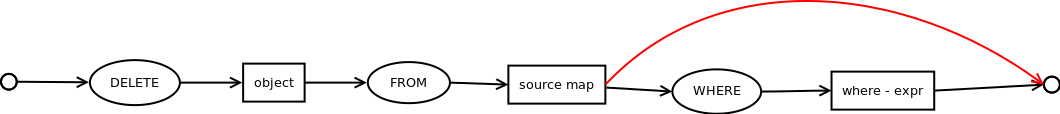
\includegraphics[scale=0.4]{images/delete}
		\caption{A DELETE lekérdezés szintaxis diagramja}
		\label{fig:deleteSytnax}
	\end{center}
\end{figure}

A szintaxis diagram alapján ezek a metódusok hívódnak meg a DeleteBuilder objektumnak:

DeleteBuilder builder = new Builder(); \\
builder.createDelete("mine"); \\ 
builder.setFrom("azeroth"); \\
builder.addOperandPiece("mine.x"); \\
builder.addOperator(">"); \\
builder.addOperandPiece("10"); \\
builder.build(); \\

Minden builder osztályban definiáltunk egy build metódust, ami egy IQueryObject példányt ad vissza. Minden lekérdezés objektum implementálja az IQueryObject interfészt, ami egy execute() metódust tartalmaz.



\section{ALTER lekérdezés felépítése}

A következő lekérdezés érkezik az adatbázismotorhoz:
\begin{sql}
ALTER CLASS Rectangle DELETEATTRIBUTE x;
\end{sql}


\begin{figure}[htb]
	\begin{center}
		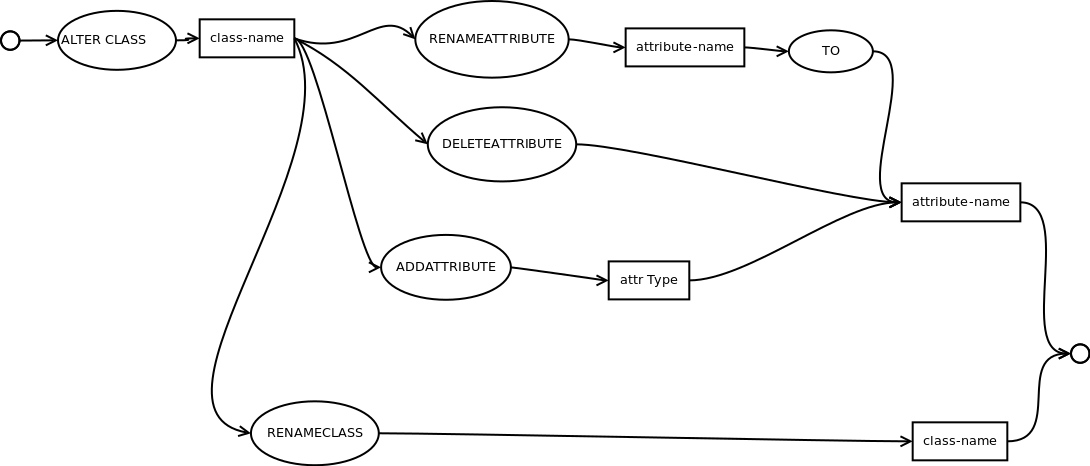
\includegraphics[scale=0.4]{images/alter}
		\caption{Az ALTER lekérdezés szintaxis diagramja}
		\label{fig:alterSytnax}
	\end{center}
\end{figure}

A builder objektum metódusainak használata a fenti lekérdezés esetében:

AlterBuilder builder = new AlterBuilder(); \\
builder.createAlter("Rectangle"); \\
builder.setAlterType("DELETEATTRIBUTE"); \\
builder.setStringAttribute("x"); \\
builder.build(); \\

Az Alter lekérdezés 4 típust definiál:

\begin{itemize}
\item Osztálynév módosítás
\item Attribútum törlés
\item Attribútum definiálás
\item Attribútum átnevezése
\end{itemize}

Ezek közül az attribútum létrehozáshoz és átnevezéshez egy plusz attribútumra van szükség, amelyet a builder.setOptionalValue(attribute-name or attribute-Type)
metódussal állíthatjuk be.

\section{CREATE lekérdezés felépítése}

A CREATE lekérdezéssel adatbázist, térképet és osztály definíciót lehet létrehozni. Az adatbázisnak és a térképnek a definiálása a legkönnyebb lekérdezések egyike, és az osztály definiálása ugyan azon lépésekből áll, csak egy párat definiál pluszba hozzájuk.

\begin{figure}[htb]
	\begin{center}
		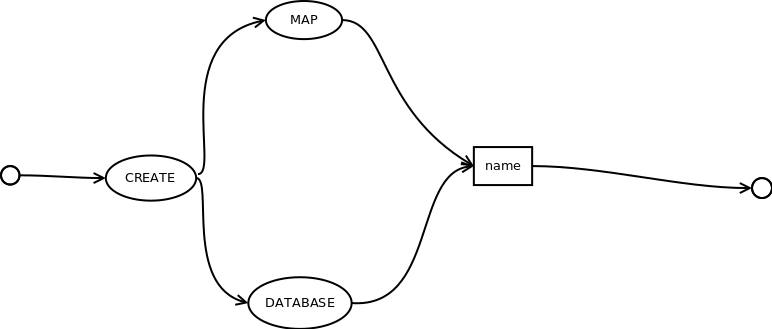
\includegraphics[scale=0.4]{images/create}
		\caption{A CREATE lekérdezés szintaxis diagramja adatbázis és térkép létrehozásra szűkítve}
		\label{fig:createSytnax}
	\end{center}
\end{figure}

\begin{figure}[htb]
	\begin{center}
		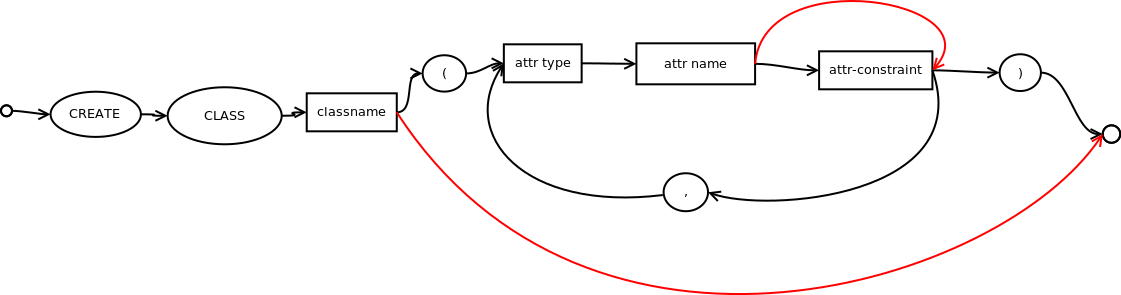
\includegraphics[scale=0.4]{images/createclass}
		\caption{A CREATE lekérdezés szintaxis diagramja osztálydefiníció definiálásához}
		\label{fig:createClassSytnax}
	\end{center}
\end{figure}



A következő lekérdezés érkezik az adatbázismotorhoz:
\begin{sql}
CREATE CLASS Harcos(
Number kor,
Number attack DEFAULT 10,
String nev);
\end{sql}

CreateBuilder builder = new CreateBuilder();
builder.setCreateType("CLASS"); \\
builder.setTheCommonValue("Harcos"); \\
builder.addAttributeParam("Number"); \\
builder.addAttributeParam("kor"); \\
builder.insertAttribute(); \\
builder.addAttributeParam("Number"); \\
builder.addAttributeParam("attack"); \\
builder.addAttributeParam("10"); \\
builder.insertAttribute(); \\
builder.addAttributeParam("String"); \\
builder.addAttributeParam("nev"); \\
builder.build(); \\

Vessző karaktereknél és a ")" karakternél hívódik meg az insertAttribute metódus, ami beszúrja az attribútumot.


\section{UPDATE lekérdezés felépítése}

A következő lekérdezés érkezik az adatbázismotorhoz:
\begin{sql}
UPDATE azeroth SET x=30,y=40 WHERE mine.id = 10;
\end{sql}

\begin{figure}[htb]
	\begin{center}
		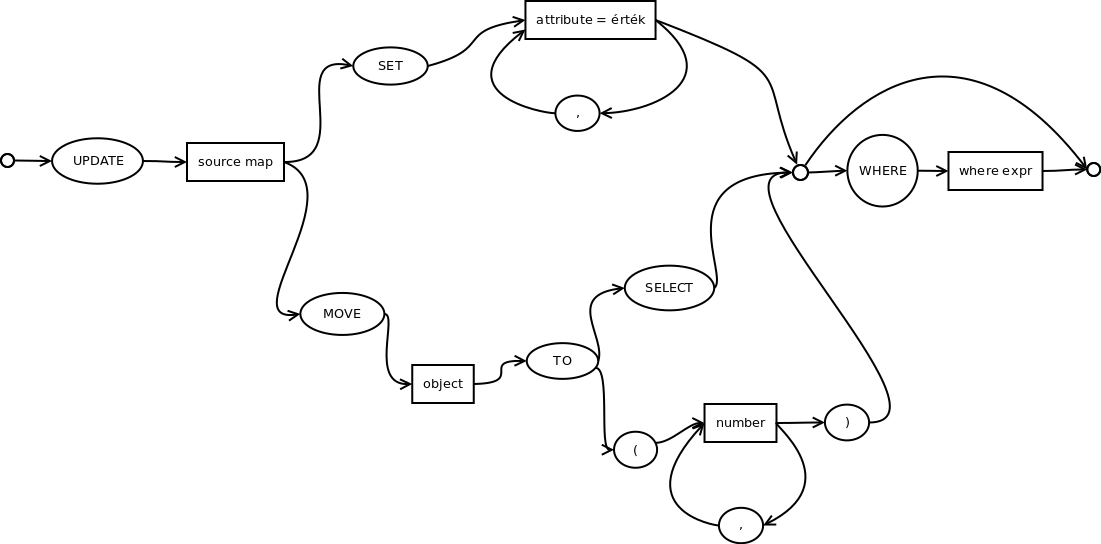
\includegraphics[scale=0.4]{images/update}
		\caption{Az UPDATE lekérdezés szintaxis diagramja}
		\label{fig:updateSytnax}
	\end{center}
\end{figure}

A parser ezeket a betódusokat hívja ebben a sorrendben ahhoz, hogy felépüljön a lekérdezés objktum:

UpdateBuilder builder = new UpdateBuilder(); \\
builder.createUpdate("azeroth"); \\
builder.setType("SET"); \\
builder.addSetAttribute("x"); \\
builder.addSetAttributeValue(30); \\
builder.addSetAttribute("y"); \\
builder.addSetAttributeValue(40); \\
builder.addOperandPiece("mine.id"); \\
builder.addOperator("="); \\
builder.addOperandPiece("10"); \\
builder.build(); \\


\section{INSERT lekérdezés felépítése}

Az Insert lekérdezés fában tárolja az objektumhoz tartozó attribútumokat. A kompozíció miatt, az attribútumok is tartalmazhatnak olyan attribútumokat, amelyek objektumok, így ezek között szülő-gyermek relációt lehet felfedezni, ezért a legegyszerűbb megoldásnak a fában való tárolás tűnt.

A  \ref{fig:insertTreeBuilder}. ábrán látható gráfokkal dolgozik az INSERT lekérdezés objektum. A jobb oldali gráf az, amire szüksége van a lekérdezés objektumnak, viszont ezt a parser nem tudja előállítani, hisz az attribútumok és az értékek el vannak különítve egymástól a lekérdezésben. Látható, hogy a két baloldali gráfból előállítható az, amelyikre az INSERT objektumnak szüksége van, ezt viszont az InsertBuilder osztály a háttérben elvégzi.



\begin{figure}[htb]
	\begin{center}
		\includegraphics[scale=0.1]{images/InsertTreeBuilder}
		\caption{Az INSERT lekérdezés adatábrázolása }
		\label{fig:insertTreeBuilder}
	\end{center}
\end{figure}


Az algoritmus az InsertBuilder gyártó osztály mögött:

A parser amikor a builder segítségével felépíti a lekérdezésobjektumot, akkor igazából a háttérben két listát tölt fel, majd a builder fogja felépíteni az objektumot a háttérben. Azért van szükség két listára, mert a lekérdezésben az attribútumok leírása, és az értékek megadása elválasztva szerepel, és így nem lehet egy metódusban létrehozni az attribútumokat. 

Az Insert osztályon belül található egy TreeBuilder osztály, amely TreeNode csomópontokat tárol, és építi fel őket.
Amikor az InsertBuilder metódusai kívülről meghívódnak, ő az Insertből példányosított objektumnak a TreeBuilder metódusait hívja tovább.

Attribútum lista: Ebben a listában tárolom az attribútumokat sorrendben, metaadatként tárolva azt, hogy beszúrást követően a fában a szülő felé kell-e lépni, és ha igen, akkor hány szintet.A \ref{fig:insertTreeBuilder}. ábrán látható gráfok közül ez a lista a bal felső sarokban lévőt tárolja.

Érték lista: Ebben a listában tárolom a VALUES kulcsszó után feltüntetett értékeket. A \ref{fig:insertTreeBuilder}. ábrán látható gráfok közül ez a lista a bal alsó sarokban lévőt tárolja.

Az attribútum és az érték lista is egyaránt ugyan annyi elemet tárol, és ha mindkettőt feltöltötte a parser, akkor az összeillesztésükhöz már csak egy iterációt kell megvalósítani, és a builder tovább tud hívni az INSERT objektum felé úgy, hogy attribútumot, és mellé értéket is párosít.

\begin{figure}[htb]
	\begin{center}
		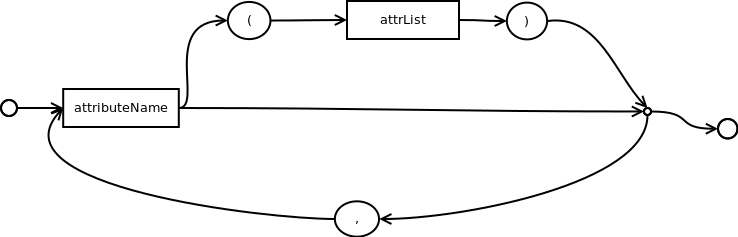
\includegraphics[scale=0.4]{images/attrList}
		\caption{Az INSERT szintaxis diagram attrList komponense}
		\label{fig:attrListSytnax}
	\end{center}
\end{figure}

\begin{figure}[htb]
	\begin{center}
		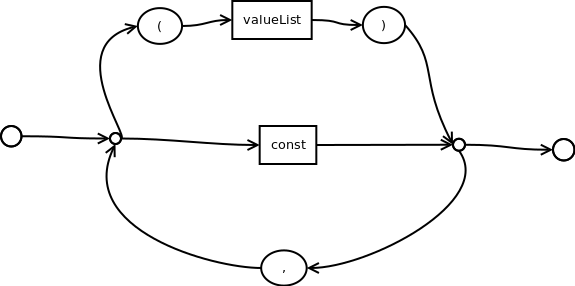
\includegraphics[scale=0.4]{images/valueList}
		\caption{Az INSERT szintaxis diagram valueList komponense}
		\label{fig:valueListSytnax}
	\end{center}
\end{figure}

\begin{figure}[htb]
	\begin{center}
		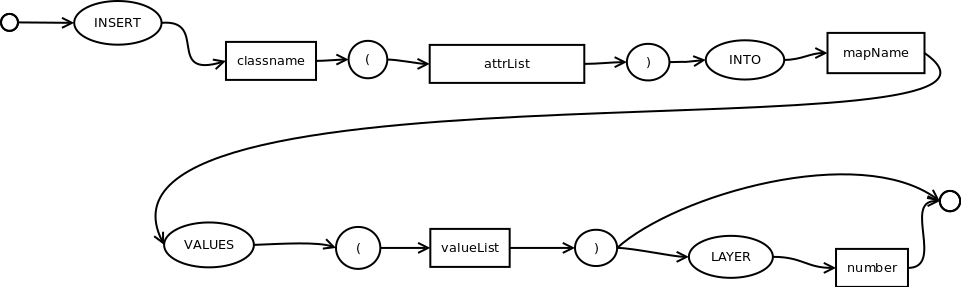
\includegraphics[scale=0.4]{images/insert}
		\caption{Az INSERT lekérdezés szintaxis diagramja}
		\label{fig:insertSytnax}
	\end{center}
\end{figure}


\section{DROP lekérdezés felépítése}

A DropBuilder implementálásakor semmilyen bonyodalomba nem ütköztünk.

\begin{figure}[htb]
	\begin{center}
		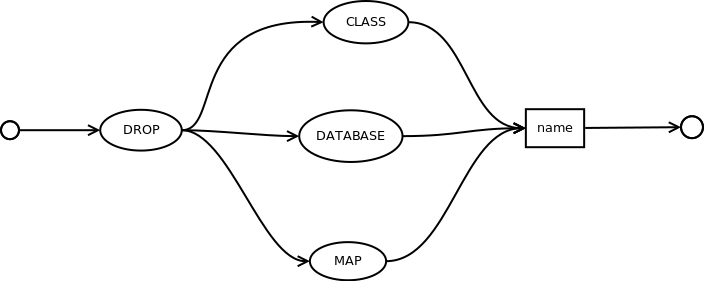
\includegraphics[scale=0.4]{images/drop}
		\caption{A DROP lekérdezés szintaxis diagramja}
		\label{fig:dropSytnax}
	\end{center}
\end{figure}

\section{Számítások optimalizálása}

Az adatbázismotor feladata levenni a terhet a felhasználó válláról, 
optimalizált algoritmusokkal támogatni a lekérdezéseket. Térképfelosztás, pályaelem összevonás, ezek mind olyan feladatok,
amelyek a térképműveletek gyorsabb végrehajtását idézik elő.
Mivel a dolgozatnak egyenlőre nem célja, hogy a piacon versenyképes szoftver legyen, ezért az optimalizálás nem került bele a dolgozatba.


